\documentclass{article}

\usepackage[T1]{fontenc}
\usepackage[utf8]{inputenc}
\usepackage[brazilian]{babel}
\usepackage{graphicx}
\usepackage[export]{adjustbox}[2011/08/13]
\usepackage{float}
\usepackage[pdftex]{hyperref}
\usepackage{epstopdf}
\usepackage{etoolbox}
\usepackage{amsmath}
\usepackage{amsfonts}
\usepackage{amssymb}
\usepackage{caption}
\usepackage{subcaption}
\usepackage{setspace}
\usepackage{tikz}
\usepackage{listings}
\usepackage{xcolor} 
\usepackage{multirow}
\usepackage{longtable}

\patchcmd{\thebibliography}{\section*}{\section}{}{}
\newcommand{\R}{\ensuremath{\mathbb{R}}}
\newcommand{\Prob}{\ensuremath{\mathbb{P}}}
\newcommand{\K}{\ensuremath{\mathbb{K}}}
\newcommand{\U}{\ensuremath{\mathbb{U}}}
\newcommand{\N}{\ensuremath{\mathbb{N}}}
\newcommand{\Lg}{\ensuremath{\mathbb{L}}}
\newcommand{\T}{\ensuremath{\rm Tr}}
\newcommand{\sg}{{\sigma(x_k)}}

\newcommand{\G}{\ensuremath{\mathcal{G}}}
\newcommand{\F}{\ensuremath{\mathcal{F}}}
\newcommand{\C}{\ensuremath{\mathcal{C}}}
\newcommand{\E}{\ensuremath{\mathcal{E}}}
\newcommand{\Hn}{\ensuremath{\mathcal{H}}}
%\newcommand{\Hoo}{\ensuremath{\mathcal{H}_\infty}}
\newcommand{\Hop}{\ensuremath{\mathcal{H}_{op}}}
% --------------------------------------------------
\newtheorem{theo}{Teorema}
\newtheorem{exa}{Exemplo}
\newtheorem{lemm}{Lema}
\newtheorem{coro}{Corolário}
\newtheorem{defn}{Definição}[section]

%opening
\lstset{ %
	backgroundcolor=\color{white},   % choose the background color; you must add \usepackage{color} or \usepackage{xcolor}
	basicstyle=\fontsize{8}{10}\ttfamily\color{black},        % the size of the fonts that are used for the code
	breakatwhitespace=true,         % sets if automatic breaks should only happen at whitespace
	breaklines=true,                 % sets automatic line breaking
	captionpos=t,                    % sets the caption-position to bottom
	commentstyle=\color{green},    % comment style
	extendedchars=true,              % lets you use non-ASCII characters; for 8-bits encodings only, does not work with UTF-8
	frame=tb,                    % adds a frame around the code
	keepspaces=true,                 % keeps spaces in text, useful for keeping indentation of code (possibly needs columns=flexible)
	keywordstyle=\color{cyan},       % keyword style
	language=C,                 % the language of the code
	numbers=left,                    % where to put the line-numbers; possible values are (none, left, right)
	numbersep=5pt,                   % how far the line-numbers are from the code
	numberstyle=\tiny\color{black}, % the style that is used for the line-numbers
	rulecolor=\color{gray},         % if not set, the frame-color may be changed on line-breaks within not-black text (e.g. comments (green here))
	showspaces=false,                % show spaces everywhere adding particular underscores; it overrides 'showstringspaces'
	showstringspaces=false,          % underline spaces within strings only
	showtabs=false,                  % show tabs within strings adding particular underscores
	stepnumber=1,                    % the step between two line-numbers. If it's 1, each line will be numbered
	stringstyle=\color{red},     % string literal style
	tabsize=2,                       % sets default tabsize to 2 spaces
}

\makeatletter
\def\code{\@ifnextchar[{\@with}{\@without}}%
\def\@with[#1]#2{%
}
\def\@without#1{%
	\subsection{\protect\detokenize{#1}}%
	\lstinputlisting[language=C, linewidth=1.3\linewidth]{#1}%
	\pagebreak%
}
\makeatother

\begin{document}
\input{capa.tex}

\onehalfspacing
\section{Objetivo} 
O objetivo do projeto é, de maneira incremental, planejar, montar e implementar um veículo robótico seguidor de linha \ref{fig:robo}. Inicialmente planejar todo o projeto através do Rational Rhapsody Modeler, em seguida, construir as placas eletrônicas e unificar os componentes mecânicos, por fim, implementar o controlador do sistema através do \textit{target}. 

\begin{figure}[H]
	\centering
	\includegraphics[width=0.9\linewidth]{carrinho.JPG}
	\caption{Veículo robótico seguidor de linha}
	\label{fig:robo}
\end{figure}
	
\section{Modelagem}
% Diagramas requisitos implementados, digrama de blocos, etc
Utilizando o Rational Rhapsody Modeler e tomando como base os requisitos propostos mostrados na figura \ref{fig:requisitos}, modelamos nossos sistema. Nessa etapa inicial nos preocupamos em detalhar como funcionaria cada componente do software e como estes interagem entre si, as figuras \ref{fig:pacotes} e \ref{fig:blocos} nos permitem ter uma visão geral dos módulos do sistema.
\begin{figure}[H]
	\centering
	\includegraphics[width=1.3\linewidth, center]{requisitos}
	\caption{Diagrama de requisitos}
	\label{fig:requisitos}
\end{figure}
\begin{figure}[H]
	\centering
	\includegraphics[width=0.9\linewidth]{pacotes}
	\caption{Diagrama de pacotes}
	\label{fig:pacotes}
\end{figure}
\begin{figure}[H]
	\centering
	\includegraphics[width=1.5\linewidth, center]{blocos}
	\caption{Diagrama de definição de blocos}
	\label{fig:blocos}
\end{figure}

Os blocos \textit{Line\_PhotoSensor\_hal}, \textit{encoder\_hal}, \textit{motor\_hal} e \textit{rgb\_led\_hal} fazem a interface entre o hardware e o software, possuindo funções para o controle dos atuadores ou a medição dos sensores. No bloco \textit{encoder\_hal} encontramos mais operações que nos outros devido à algumas particularidades do sistema. Escolhemos separar a requisição de leitura dos encoders da obtenção dos resultados para facilitar o reaproveitamento da mesma leitura em mais de um local do ciclo executivo cooperativo, fizemos issso através das funções \textit{measure} e \textit{getCurrentSpeed}/\textit{getLinDistance}. Notamos que a precisão de nossos encoders não é alta o suficiente para obter uma medida de velocidade razoável dentro do período do nosso ciclo executivo padrão, para resolver essa dificuldade utilizamos a função \textit{getMeanSpeed} que nos retorna uma média das últimas medidas (mantidas em um buffer circular), essa solução, embora introduza um atraso no sistema, nos permite manter o período do ciclo executivo relativamente baixo.

O bloco \textit{Line\_Sensor} é responsável por obter as medidas de luminosidade dos foto-sensores e converte-las na posição do centro da linha, isto é feito através do algoritmo spline, detalhes do seu funcionamento são apresentados nas figura \ref{fig:lineMeasure}. Ele também avisa nossa máquina de estados quando um sinal de comando de linha é encontrado. O bloco \textit{SpeedController} é responsável pelo controle de velocidade do carrinho, ele recebe uma velocidade linear e angular de referência e executa o controle dos motores em malha fechada utilizando a medida dos encoders. Já o bloco \textit{Line\_Controller} é responsável por seguir a linha, este requisita medições do centro de linha do \textit{Line\_Sensor} e calcula as velocidades de referência que deverão ser passadas para o \textit{SpeedController}, um esquema geral do seu funcionamento pode ser visto nas figuras \ref{fig:stateLine}, \ref{fig:lineMeasure} e \ref{fig:line}

\begin{figure}[H]
	\centering
	\includegraphics[width=0.9\linewidth]{stateLine}
	\caption{Diagrama de Máquina de Estados do controlador de linha}
	\label{fig:stateLine}
\end{figure}
\begin{figure}[H]
	\centering
	\includegraphics[width=0.9\linewidth]{stateLineMeasure}
	\caption{Diagrama de Sub Máquina de Estados - Sensor de linha}
	\label{fig:lineMeasure}
\end{figure}
\begin{figure}[H]
	\centering
	\includegraphics[width=0.9\linewidth]{line}
	\caption{Diagrama de Sequência - Controlador de Linha}
	\label{fig:line}
\end{figure}

O bloco \textit{AutoTest} tem como função o teste e calibração do sistema, testando primeiramente se os motores e foto-sensores estão funcionando para em seguida calibrá-los. Seu funcionamento encontra-se detalhado nas figuras \ref{fig:stateAutoTeste}, \ref{fig:testIR}, \ref{fig:testMotor} e \ref{fig:testes}.

\begin{figure}[H]
	\centering
	\includegraphics[width=0.9\linewidth]{stateAutoTeste}
	\caption{Diagrama de Máquina de Estados do módulo de Auto-Teste}
	\label{fig:stateAutoTeste}
\end{figure}
\begin{figure}[H]
	\centering
	\includegraphics[width=0.9\linewidth]{testIR}
	\caption{Diagrama de Sub Máquina de Estados - Teste dos Sensores infra-vermelhos}
	\label{fig:testIR}
\end{figure}
\begin{figure}[H]
	\centering
	\includegraphics[width=0.9\linewidth]{testMotor}
	\caption{Diagrama de Sub Máquina de Estados - Teste dos Motores e Encoders}
	\label{fig:testMotor}
\end{figure}
\begin{figure}[H]
	\centering
	\includegraphics[width=0.9\linewidth]{testes}
	\caption{Diagrama de Sequência - Módulo de Auto-Teste e calibração}
	\label{fig:testes}
\end{figure}

O bloco \textit{stateMachine} lida com a interpretação dos comandos e ativação dos outros módulos do sistema (Acertando a velocidade linear de referência que será passada ao nosso controlador de lina). A máquina de estados do tratamento dos comandos pode ser vista na figura \ref{fig:estados}.

\begin{figure}[H]
	\centering
	\includegraphics[width=0.9\linewidth]{stateMachine}
	\caption{Diagrama de máquina de estados para interpretação dos comandos}
	\label{fig:estados}
\end{figure}

Nos estados normal e walk o nosso controlador de linha receberá uma velocidade linear de referência relativamente baixa (em torno de 50\% da velocidade máxima do sistema), quando estamos no estado maxSpeed essa referência será maior (95\%) e em stop ela será nula.

O diagrama de atividades apresentado na figura \ref{fig:main} sintetiza o sistema como um todo, mostrando sua execução através do modelo cíclico executivo cooperativo.

\begin{figure}[H]
	\centering
	\includegraphics[width=0.9\linewidth]{atividades}
	\caption{Diagrama de atividades do sistema}
	\label{fig:main}
\end{figure}

\section{Matriz de Rastreabilidade}
A matriz de rastreabilidade apresentada na tabela \ref*{tab:rastreabilidade} relaciona cada um dos requisitos com a sua implementação.
\pagebreak
\small
\begin{longtable}{|p{0.125\linewidth}|p{0.17\linewidth}|p{0.75\linewidth}|}
\hline \bfseries{Requisito} & \bfseries{SubRequisito} & \bfseries{Implementação}\\ 
		\hline 
        \multirow{2}{*}{REQ1}
        & REQ1.A & \texttt{autotest.c}\\ 
        && \texttt{- void autotest\_testAndCalibrate(void)}\\
        && \texttt{- void autotest\_testPhotoSensors(void)}\\
		\cline{2-3}
        & REQ1.B & \texttt{autotest.c}\\ 
        && \texttt{- void autotest\_testAndCalibrate(void)}\\
        && \texttt{- void autotest\_testPhotoSensors(void)}\\
        \cline{2-3}
        & REQ1.C & \texttt{autotest.c}\\ 
        && \texttt{- void autotest\_testAndCalibrate(void)}\\
        && \texttt{- void autotest\_testPhotoSensors(void)}\\
		\cline{2-3}
        & REQ1.D & \texttt{autotest.c}\\ 
        && \texttt{- void autotest\_testAndCalibrate(void)}\\
        && \texttt{- void autotest\_testPhotoSensors(void)}\\
        \cline{2-3}
        & REQ1.E & \texttt{autotest.c}\\ 
        && \texttt{- void autotest\_testAndCalibrate(void)}\\
        && \texttt{- void autotest\_testPhotoSensors(void)}\\
		\cline{2-3}
        & REQ1.F & \texttt{autotest.c}\\ 
        && \texttt{- void autotest\_testAndCalibrate(void)}\\
        && \texttt{- void autotest\_testPhotoSensors(void)}\\
		\cline{2-3}
        & REQ1.G & \texttt{autotest.c}\\ 
        && \texttt{- void autotest\_testAndCalibrate(void)}\\
        && \texttt{- void autotest\_testMotors()}\\
		\cline{2-3}
        & REQ1.H & \texttt{autotest.c}\\ 
        && \texttt{- void autotest\_testAndCalibrate(void)}\\
        && \texttt{- void autotest\_testMotors()}\\
        \hline
        \multirow{2}{*}{REQ2}
        & REQ2.A & \texttt{autotest.c}\\ 
        && \texttt{- void autotest\_testAndCalibrate(void)}\\
        && \texttt{- void autotest\_calibratePhotoSensors(void)}\\
        && \texttt{photosensor\_hal.c}\\
        && \texttt{- void photoSensor\_calibrate(unsigned short usSensorNumber, int iLightVal, int iDarkVal)}\\
		\cline{2-3}
        & REQ2.B & \texttt{autotest.c}\\ 
        && \texttt{- void autotest\_testAndCalibrate(void)}\\
        && \texttt{- void autotest\_calibratePhotoSensors(void)}\\
        && \texttt{photosensor\_hal.c}\\
        && \texttt{- void photoSensor\_calibrate(unsigned short usSensorNumber, int iLightVal, int iDarkVal)}\\
        \cline{2-3}
        & REQ2.C & \texttt{autotest.c}\\ 
        && \texttt{- void autotest\_testAndCalibrate(void)}\\
        && \texttt{- void autotest\_calibratePhotoSensors(void)}\\
        && \texttt{photosensor\_hal.c}\\
        && \texttt{- void photoSensor\_calibrate(unsigned short usSensorNumber, int iLightVal, int iDarkVal)}\\
		\cline{2-3}
        & REQ2.D & \texttt{autotest.c}\\ 
        && \texttt{- void autotest\_testAndCalibrate(void)}\\
        && \texttt{- void autotest\_calibratePhotoSensors(void)}\\
        && \texttt{photosensor\_hal.c}\\
        && \texttt{- void photoSensor\_calibrate(unsigned short usSensorNumber, int iLightVal, int iDarkVal)}\\
        \cline{2-3}
        & REQ2.E & \texttt{autotest.c}\\ 
        && \texttt{- void autotest\_testAndCalibrate(void)}\\
        && \texttt{- void autotest\_calibratePhotoSensors(void)}\\
        && \texttt{photosensor\_hal.c}\\
        && \texttt{- void photoSensor\_calibrate(unsigned short usSensorNumber, int iLightVal, int iDarkVal)}\\
		\cline{2-3}
        & REQ2.F & \texttt{autotest.c}\\ 
        && \texttt{- void autotest\_testAndCalibrate(void)}\\
        && \texttt{- void autotest\_calibratePhotoSensors(void)}\\
        && \texttt{photosensor\_hal.c}\\
        && \texttt{- void photoSensor\_calibrate(unsigned short usSensorNumber, int iLightVal, int iDarkVal)}\\
		\cline{2-3}
        & REQ2.G & \texttt{autotest.c}\\ 
        && \texttt{- void autotest\_testAndCalibrate(void)}\\
        && \texttt{- void autotest\_calibrateMotors()}\\
        && \texttt{speedController.c}\\
        && \texttt{- void speedControl\_calibrate(unsigned short usMotorNumb, int iMin, unsigned int uiMax, int iInvMin, unsigned int uiInvMax)}\\
		\cline{2-3}
        & REQ2.H & \texttt{autotest.c}\\ 
        && \texttt{- void autotest\_testAndCalibrate(void)}\\
        && \texttt{- void autotest\_calibrateMotors()}\\
        && \texttt{speedController.c}\\
        && \texttt{- void speedControl\_calibrate(unsigned short usMotorNumb, int iMin, unsigned int uiMax, int iInvMin, unsigned int uiInvMax)}\\
        \hline
        \multirow{2}{*}{REQ3}
        & REQ3.A & \texttt{speedController.c}\\ 
        && \texttt{- void speedControl\_init(unsigned int uiKp[2], unsigned int uiKi[2], unsigned int uiKd[2], unsigned int sampleTime)}\\
        && \texttt{- void speedControl\_execute(int iLinSpeed, int iAngSpeed)}\\
		\cline{2-3}
        & REQ3.B & \texttt{speedController.c}\\ 
        && \texttt{- void speedControl\_init(unsigned int uiKp[2], unsigned int uiKi[2], unsigned int uiKd[2], unsigned int sampleTime)}\\
        && \texttt{- void speedControl\_execute(int iLinSpeed, int iAngSpeed)}\\
        \hline
         \multirow{2}{*}{REQ4}
        & REQ4.A & \texttt{encoder\_hal.c}\\ 
        && \texttt{- void encoder\_init(void)}\\
        && \texttt{- void encoder\_measure()}\\
        && \texttt{- unsigned int encoder\_getCurrentSpeed(unsigned short usEncoderNumber, unsigned int uiPeriod)}\\
        && \texttt{- unsigned int encoder\_getMeanSpeed(unsigned short usEncoderNumber, unsigned int uiPeriod)}\\
        && \texttt{- unsigned int encoder\_getLinDistance()}\\
		\cline{2-3}
        & REQ4.B & \texttt{encoder\_hal.c}\\ 
        && \texttt{- void encoder\_init(void)}\\
        && \texttt{- void encoder\_measure()}\\
        && \texttt{- unsigned int encoder\_getCurrentSpeed(unsigned short usEncoderNumber, unsigned int uiPeriod)}\\
        && \texttt{- unsigned int encoder\_getMeanSpeed(unsigned short usEncoderNumber, unsigned int uiPeriod)}\\
        && \texttt{- unsigned int encoder\_getLinDistance()}\\
        \hline
         \multirow{2}{*}{REQ5}
        & REQ5.A & \texttt{motor.c}\\ 
        && \texttt{- void motor\_init(void)}\\
        && \texttt{- void motor\_setSpeed(unsigned short usMotorNumber, int iSpeed)}\\
		\cline{2-3}
        & REQ5.B & \texttt{motor.c}\\ 
        && \texttt{- void motor\_init(void)}\\
        && \texttt{- void motor\_setSpeed(unsigned short usMotorNumber, int iSpeed)}\\
		\hline
        REQ6 & - & \texttt{stateMachine.c}\\
         && \texttt{- void stateMachine\_foundCommand(unsigned short usFoundCommand)}\\
         && \texttt{lineSensor·c}\\
         && \texttt{- int lineSensor\_measure()}\\
         \hline
         REQ7 & - & \texttt{stateMachine.c}\\
         && \texttt{- void stateMachine\_execute(int iMeasuredDistance, unsigned int uiTime))}\\
         \hline
		 REQ8 & - & \texttt{lineSensor·c}\\
         && \texttt{- int lineSensor\_measure()}\\
         && \texttt{photosensor\_hal.c}\\
         && \texttt{- unsigned short photoSensor\_measure(unsigned short usSensorNumber)}\\
         \hline
         REQ9 & - & \texttt{lineControl·c}\\
         && \texttt{- void lineControl\_init(unsigned int uiKp, unsigned int uiKi, unsigned int uiKd, unsigned int sampleTime)}\\
         && \texttt{- void lineControl\_execute(int iLinSpeed)}\\
         \hline
    \caption{Matriz de Rastreabilidade}
	\label{tab:rastreabilidade}
\end{longtable}
\normalsize



\section{Montagem eletrônica e mecânica}
% montagens
Seguindo o modelo sugerido pela figura \ref{fig:sensoresEsq} montamos a placa de sensores \ref{fig:led}. A placa de sensores é um componente elétrico que faz as medidas de posição do veículo, através de 6 pares de emissor/receptor de infra-vermelho. Cada par é separado fisicamente em 10mm. Essa distância é selecionada para que cada não haja grande interferência, a distância é interessante também para a computação da posição, já que, o tamanho da linha a ser seguida possui por volta deste valor.
A placa de sensores de posição foi integrada à placa geral de controle, para isso através de conectores KK. A alimentação do circuito lógico foi realizada através de um Powerbank.

\begin{figure}[H]
	\centering
	\includegraphics[width=0.9\linewidth]{sensoresEsq}
	\caption{Diagrama esquemático da placa de sensores infra-vermelhos}
	\label{fig:sensoresEsq}
\end{figure}

\begin{figure}[H]
	\centering
	\includegraphics[width=0.9\linewidth]{led.JPG}
	\caption{Placa de sensores infra-vermelhos}
	\label{fig:led}
\end{figure}
Como os receptores produzem um sinal analógico, for necessária a utilização de ADCs para a leitura dos mesmos, para isso utilizamos as portas as portas PTB0, PTB1, PTB2, PTE20, PTE21 e PTE22 do target, configuradas,respectivamente, como ADC0\_SE8, ADC0\_SE9, ADC0\_SE12, ADC0\_SE0, ADC0\_SE4a, ADC0\_SE3. Já os emissores são acionados por portas GPIO, utilizamos as portas PTA16, PTA17, PTC13, PTC16, PTC17, e PTE31 configuradas como saídas GPIO. Para a aquisição dos sinais de entrada configuramos nosso módulo ADC para trabalhar com conversões de 16-bit, com tempo de amostragem curto e utilizando o recurso de média por hardware, configurada para 32 amostras por leitura. Calculamos o tempo de computação dessas medidas e vimos que estamos dentro do tempo aceitável para nosso ciclo executivo.

A montagem mecânica compreende a interligação dos encoders com o motor e a placa geral de controle  \ref{fig:motor}. Para isso foi utilizada uma ponte H L293, \ref{fig:l293}, e uma alimentação própria, 4 pilhas AA em série. 

\begin{figure}[H]
	\centering
	\includegraphics[width=0.9\linewidth]{motor.JPG}
	\caption{Motores e enconder}
	\label{fig:motor}
\end{figure}

\begin{figure}[H]
	\centering
	\includegraphics[width=0.9\linewidth]{l293.jpg}
	\caption{Ponte H L293}
	\label{fig:l293}
\end{figure}

A ponte H permite o usuário controlar a velocidade e a direção de rotação dos motores. Esse controle é feito através de dois pinos GPIO e um sinal de PWM para cada motor. Através dos pinos GPIO, conectados esses aos pinos 1/3A e 2/4A da ponte H, selecionamos a direção de rotação e com o sinal PWM, conectado no pino enable, definimos a velocidade. Desta forma foi selecionado as seguintes portas para o motor 1: PTC4 e PTC7 como GPIO e PTA13 (configurado como FTM1\_CH1) como PWM, já para o motor 2: PTC0 e PTC3 como GPIO e PTA12 (configurado como FTM1\_CH0) como PWM. As saídas 1Y e 2Y da ponte H foram conectadas à alimentação do motor 1 e as saídas 3Y e 4Y à alimentação do motor 2. O diagrama lógico das entradas e saídas do IC pode ser visto na figura \ref{fig:logicPonteH}

\begin{figure}[H]
	\centering
	\includegraphics[width=0.6\linewidth]{logicPonteH}
	\caption{Diagrama Lógico da Ponte H L293 \cite{bb:l293}}
	\label{fig:logicPonteH}
\end{figure}

Para a montagem eletrônica dos encoders utilizamos o esquemático da figura \ref{fig:encoder1} como referência. A tensão de alimentação foi dimínuída para $3.3V$ e as resistências foram dimensionadas de acordo com a datasheet \cite{bb:photo}, assumindo os mesmos valores utilizados na placa de sensores. A saída dos encoders foram conectadas nas portas PTE29 e PTE30, configuradas como FTM\_CLKIN0 e FTM\_CLKIN1 respectivamente, dessa maneira utilizamos essas duas portas como o clock de referência para os módulos TPM2 e TPM0.

\begin{figure}[H]
	\centering
	\includegraphics[width=0.6\linewidth]{encoder1}
	\caption{Diagrama esquemático para placa de encoder}
	\label{fig:encoder1}
\end{figure}

\section{Teste de funcionalidade}

Uma parte importante do projeto é testar todos os componentes e ligações elétricas. 

Ao iniciar a execução da rotina a primeira etapa do sistema é a análise da funcionalidade dos componentes, sensores e atuadores. Primeiramente é feito o teste dos infra-vermelhos, com o emissor desligado, capta-se alguns valores do receptor, gerando uma gama de dados de comparação com a etapa seguinte de emissor ligado, caso não haja real diferença entre os dois, este sistema está com defeito e deve ser averiguado. Para visualização do usuário, o LED do {target} se acende com uma cor determinada pelo infra-vermelho com falha.

Após este teste há o teste dos motores. O teste dos motores é baseado na medição dos encoders, o motor é ligado e os encoders inicializados, caso não haja medição, ou o encoder está com defeito, ou o motor é que está. Neste caso é mais fácil para o usuário verificar o defeito já que o robô se movimentará ou não. Caso haja falha do encoder, o LED do {target} se acenderá com uma cor definida pelo encoder com falha.

 
\section{Calibração dos sensores}

Feito os testes dos sensores e atuadores, é necessário realizar a calibração dos mesmos. A calibração é a definição dos valores máximos e mínimos que o sistema atuará, gerando dessa forma parâmetros que dependem de situações externas ao do robô, como por exemplo, baixa bateria, diferentes tipos de superfície e baixa ou alta luminosidade.

Como, no nosso caso, a calibração dos sensores dependerá  da funcionalidade dos motores, a calibração começa pelo motor. A calibração do motor é realizado da seguinte forma: Coloca-se o valor máximo de PWM, aguarda alguns segundos e verifica-se o valor do encoder em pulsos por milissegundo. Feito isso reduz-se gradativamente o valor do PWM até a parada do robô, tal PWM é o mínimo necessário para movimentar o robô. Com tais valores podemos realizar o controle de velocidade compatível com o que o motor pode realizar. Esse procedimento é realizado nos dois sentidos para os dois motores.

A calibração dos infra-vermelhos é realizada pelas seguintes etapas: com o emissor desligado, mede-se o valor do receptor em cima da pista clara, esse valor é um offset do sistema e deve ser retirado. Com o robô ainda em cima da pista, liga-se um dos motores, fazendo o robô girar no próprio eixo, o robô passará tanto pela superfície clara, quanto pela escura, basta então armazenar os valores máximos e mínimos para definir o intervalo de operação. Faz-se o mesmo, só que rodando no sentido oposto. O intervalor é único para cada infra-vermelho.

\section{Detecção de linha}
% falar sobre detecção e determinação da posição - spline (-25 <> 25)
Para seguir uma linha ou caminho é necessário inicialmente encontrar tal caminho e definir sua posição relativa à este. Pela largura do caminho e pelo distanciamento físico dos infra-vermelhos, haverá sempre 2 infra-vermelhos detectando a linha caso o robô esteja em cima da mesma (a resposta dos sensores varia conforme a sua posição relativa a linha, caso em cima, a resposta será baixa).

Possuindo os valores dos 6 sensores é necessário agora encontrar a real posição relativa do robô, para tal realizamos uma curva de aproximação. A opção de solução foi o algoritmo Catmull-Spline \cite{bb:spline}. Repetimos a primeira e última medida para gerar os pontos inicial e final e, uma vez ajustado o polinômio, resolvemos a equação da derivada para a determinação do ponto mínimo em cada intervalo, encontrando por fim o mínimo global da curva. O algoritmo foi implementado primeiramente em Matlab para testes e alguns de seus resultados podem ser vistos na figura \ref{fig:spline}.

\begin{figure}[H]
	\centering
	\begin{subfigure}{0.45\textwidth}
		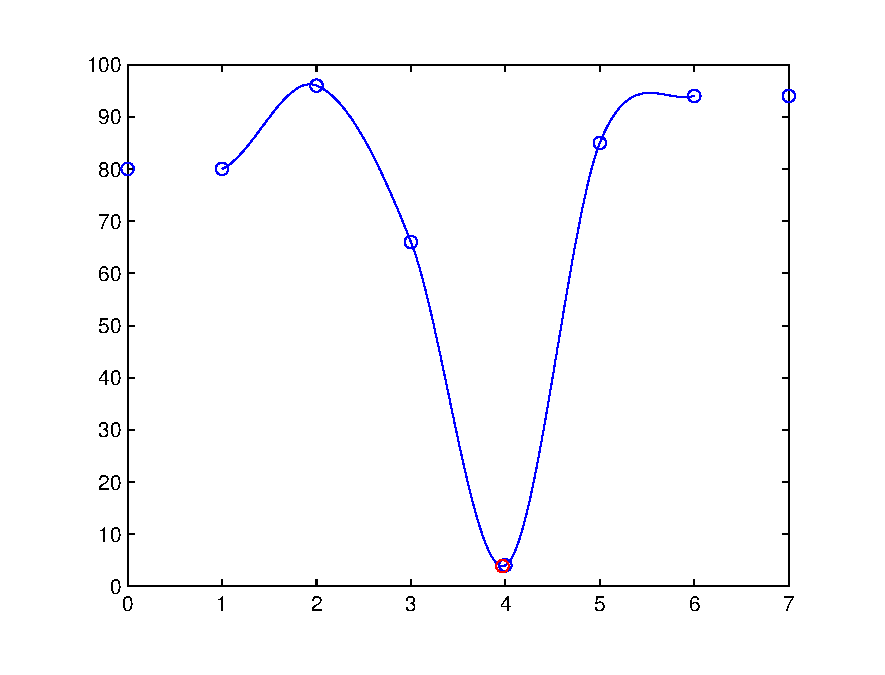
\includegraphics[width=\linewidth]{spline1}
	\end{subfigure}
	\begin{subfigure}{0.45\textwidth}
		\includegraphics[width=\linewidth]{spline2}
	\end{subfigure}
	\begin{subfigure}{0.45\textwidth}
		\includegraphics[width=\linewidth]{spline3}
	\end{subfigure}
	\caption{Resultados do algoritmo de spline simulado via Matlab}	
	\label{fig:spline}
\end{figure}


A distância entre o centro do robô até o sensor mais externo é 25mm, desta forma definimos que a posição relativa do robô varia entre -25 e 25, sendo 0 o centro. Caso o robô não esteja em cima da linha o valor de posição relativa permanece constante.

\section{Detecção de comando}

Para a detecção de comandos consideramos que quando mais do que 5 dos foto-sensores estão medindo preto é porque um sinal de comando foi encontrado, para eliminar ruídos, só levamos em consideração sinais de comando se eles foram medidos mais do que duas vezes consecutivas. Quando detectamos o primeiro sinal de comando o robô passa a procurar por um segundo, se ele percorrer uma distância pré definida sem encontrar este ele considera que recebeu o comando de velocidade máxima e aumenta sua velocidade linear de referência até que o próximo comando seja encontrado, caso contrário ele considera que recebeu o comando de parada, nesse caso ele anda uma distância pré definida e depois para por um tempo também pré definido. 

\section{Controle de velocidade}

Com a calibração dos motores e funcionalidade do encoder podemos realizar um controle de malha fechada para os dois motores separadamente afim de definir uma velocidade de cruzeiro.

A calibração nos serve para traçar uma curva de funcionalidade dos motores, verificamos qual é a velocidade máxima de cada motor e em cada direção. Como os motores são diferentes os limites máximos são diferentes, assim como o PWM mínimo para iniciar o movimento, o controlador deve atuar de forma a fornecer 2 PWMs, possivelmente diferentes, que geram a mesma velocidade linear, desta forma, movimentando o robô em linha reta.

O controlador realizado foi baseado em um PI. Os ganhos proporcionais e integrais foram encontrados com base em testes empíricos. Para definir o ganho proporcional foi verificado o tempo de resposta, via comunicação serial entre {host}-{target}, atingido um tempo satisfatório. A próxima etapa é encontrar o valor do ganho integral, para este foi analisado o erro estacionário. 

Os ganhos do controlador de velocidade são iguais para os dois motores. Apesar da diferença dos motores, como o sistema não precisa de uma precisão grande, os controladores iguais são satisfatórios.

\section{Controle de linha}

Com a calibração dos sensores infra-vermelhos e com o Catmull-Spline funcionando corretamente, podemos realizar o controle de posição do robô em relação a linha.

Possuindo a posição relativa do centro do veículo ao centro da linha, nos basta incrementar ou decrementar um dos PWM das rodas, gerando um movimento angular. O controle de posição define o quanto deve ser essa rotação.

Para o controle de posição foi realizado um controlador P. O coeficiente foi encontrado de forma empírica com base na velocidade de resposta dos motores. Neste caso, o tempo de resposta é importante para que o veículo não perca o caminho, desta forma, o proporcional é de grande importância para o sistema.

Caso o veículo perca o caminho, o mesmo buscará o caminho rotacionando para a última posição armazenada.

\begin{thebibliography}{widestlabel}
	\bibitem{bb:l293}{Texas Instruments - Datasheet: L293x Quadruple Half-H Drivers}
    \bibitem{bb:photo}{Photonic - Datasheet: CHAVES OPTOELETRÔNICAS TRANSMISSIVAS - PHCT102/3/4, PHCT202/3/4}
    \bibitem{bb:spline}{E. Catmull and R. Rom - A class of local interpolating splines}
\end{thebibliography}
\pagebreak

\end{document}

		